\documentclass[tikz,border=15pt]{standalone}
\usepackage{tikz}
\usetikzlibrary{shapes,arrows.meta,positioning,fit,backgrounds,calc}
\usepackage{amsmath,amssymb}
\usepackage{times}

\begin{document}
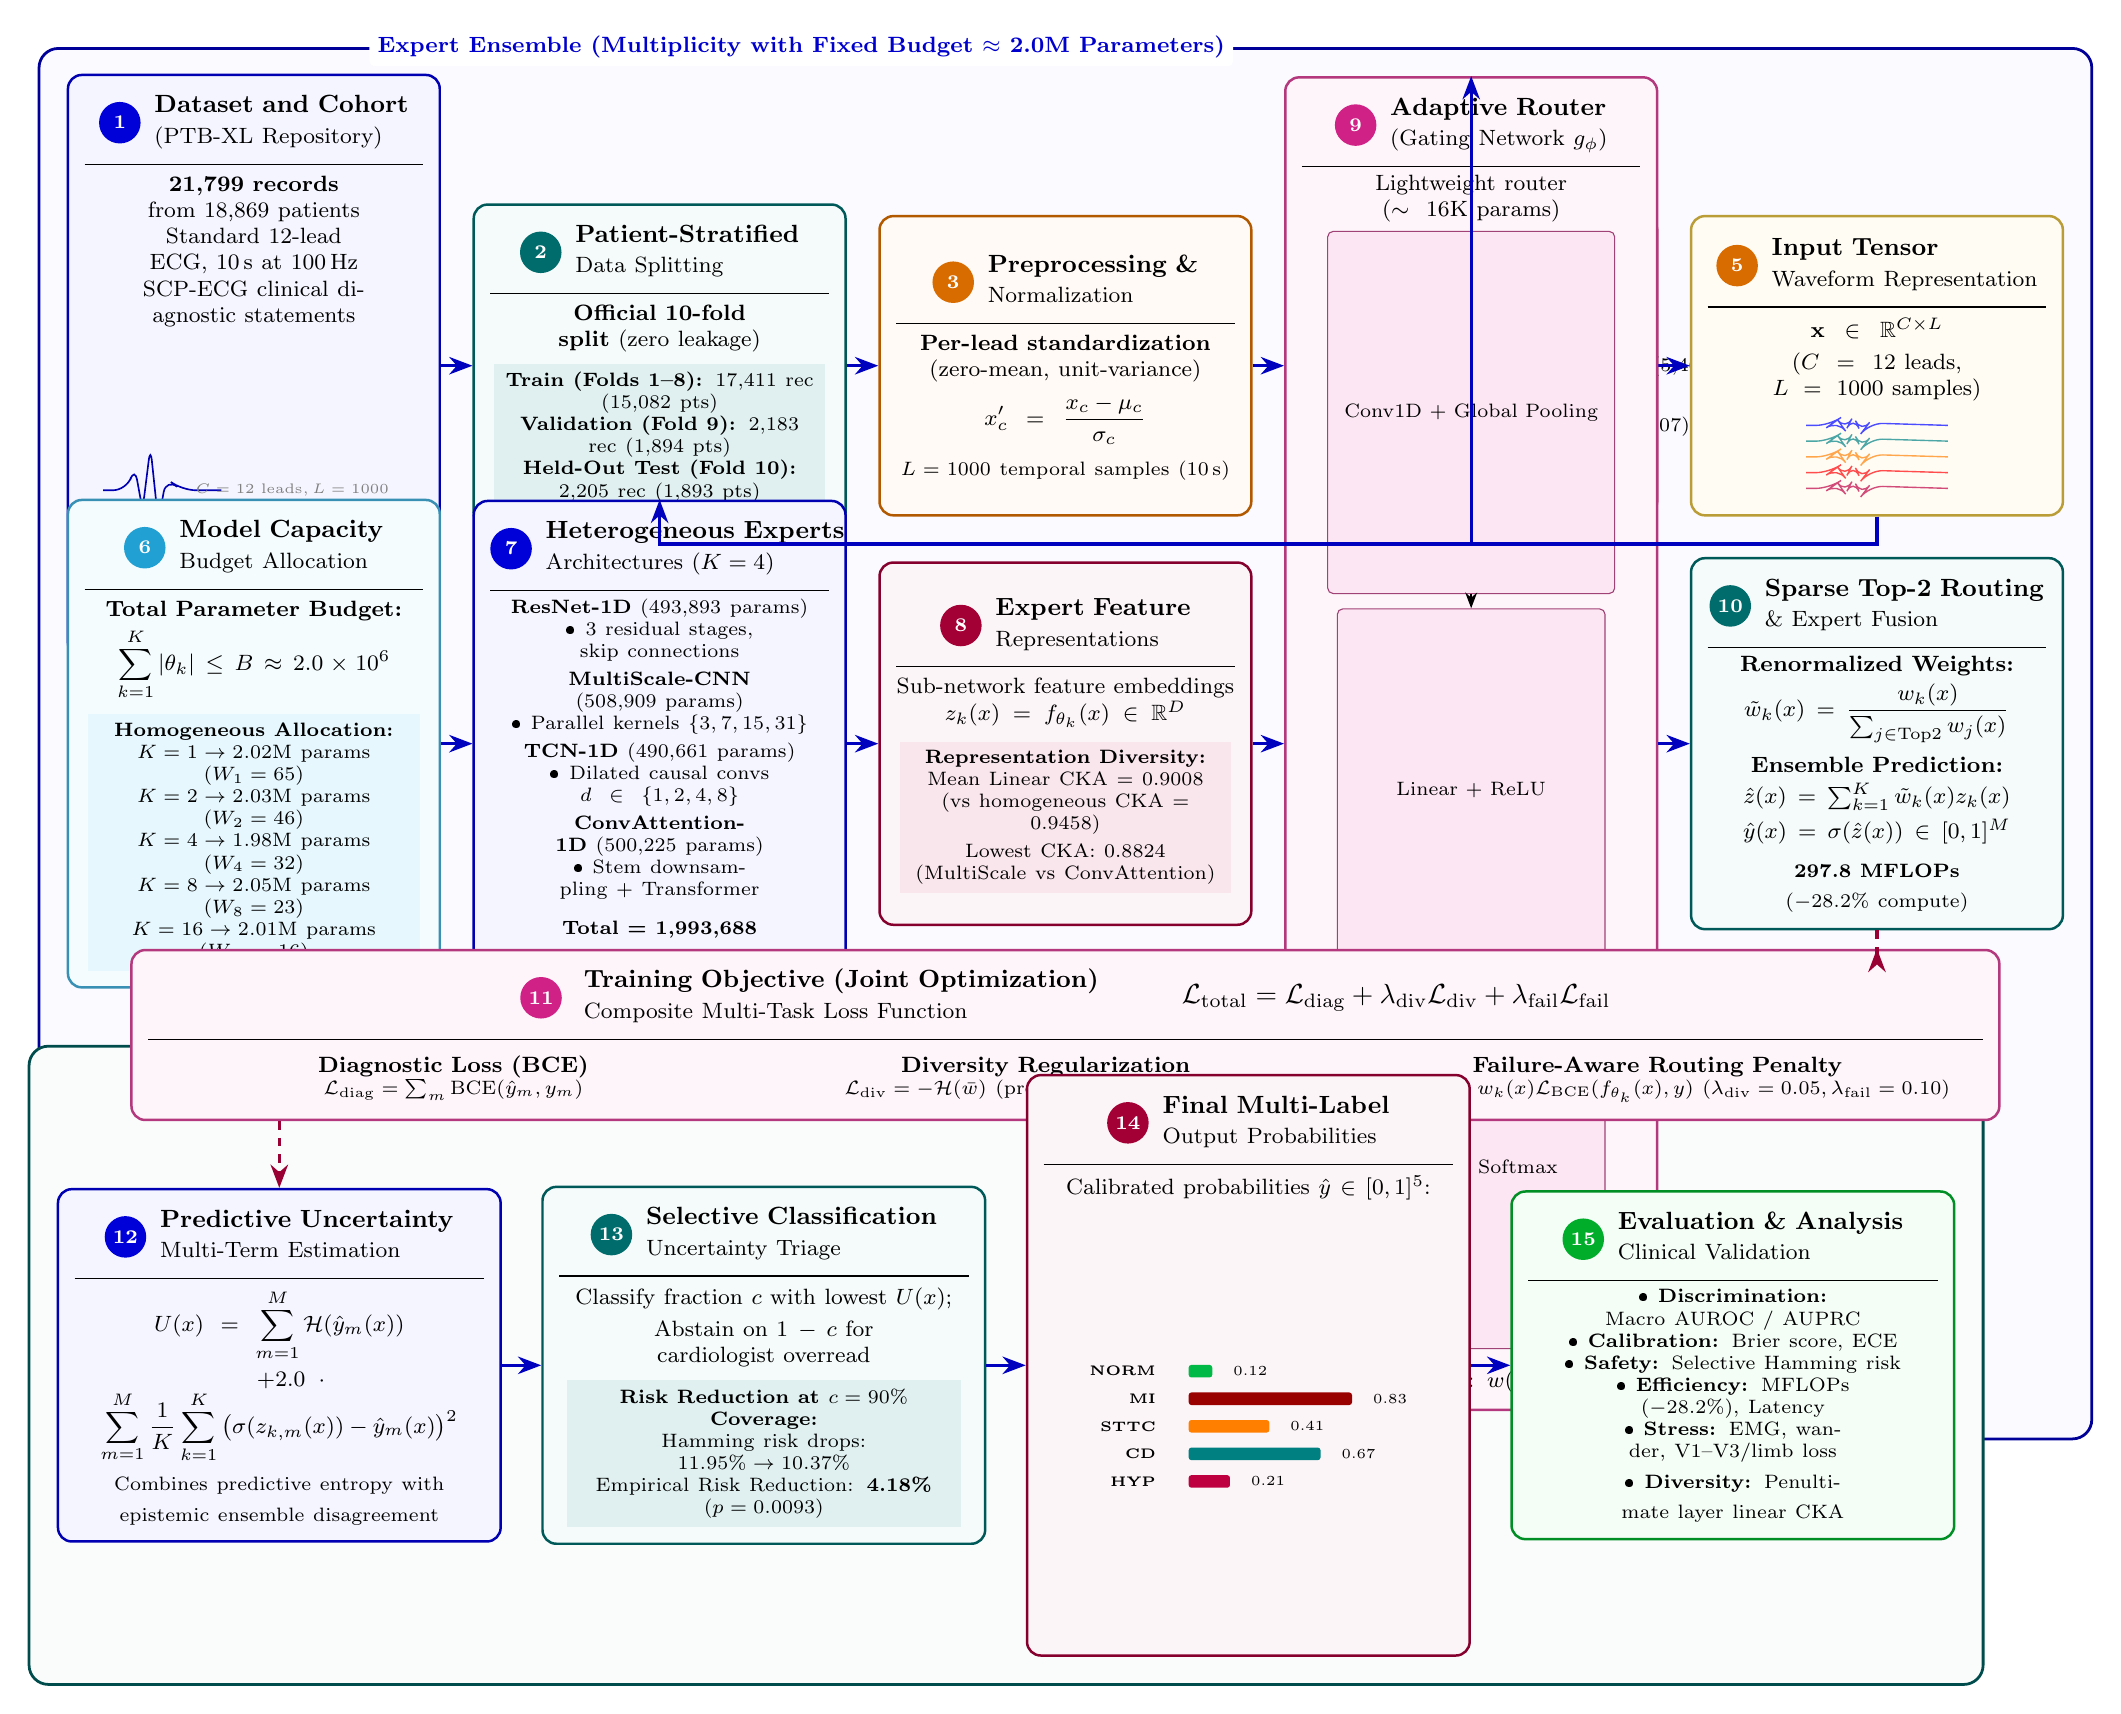
\begin{tikzpicture}[
    font=\small,
    >=Stealth,
    % Box Styles
    box/.style={
        rectangle, 
        rounded corners=5pt, 
        draw=#1!70!black, 
        fill=#1!4, 
        line width=0.9pt, 
        inner sep=6pt, 
        align=center
    },
    headerbox/.style={
        rectangle, 
        rounded corners=3pt, 
        draw=none, 
        fill=#1!15, 
        inner sep=3pt,
        text=#1!90!black,
        font=\bfseries\footnotesize,
        align=left
    },
    badge/.style={
        circle, 
        fill=#1!85!black, 
        text=white, 
        font=\bfseries\scriptsize, 
        inner sep=0pt, 
        minimum size=15pt,
        align=center
    },
    arr/.style={
        ->, 
        line width=1.2pt, 
        draw=blue!75!black
    },
    dasharr/.style={
        ->, 
        dashed, 
        line width=1.2pt, 
        draw=purple!80!black
    },
    groupframe/.style={
        rectangle, 
        rounded corners=7pt, 
        draw=#1!60!black, 
        fill=#1!2, 
        line width=1.0pt, 
        inner sep=10pt
    }
]

% =========================================================================
% TIER 1: DATA PIPELINE (Boxes 1 to 5)
% =========================================================================

% Coordinate origins for 5 columns
\def\colw{4.6cm}
\def\t1h{3.8cm}

% Box 1: Dataset & Cohort
\node[box=blue, text width=4.3cm, minimum height=\t1h] (b1) at (0, 0) {
    \begin{tabular}{@{}c@{\hspace{5pt}}l@{}}
        \tikz[baseline=-2pt]{\node[badge=blue]{1};} & 
        \begin{tabular}[c]{@{}l@{}}\textbf{Dataset and Cohort}\\\footnotesize (PTB-XL Repository)\end{tabular}
    \end{tabular}\\[4pt]
    \hrule height 0.4pt\vspace{4pt}
    \footnotesize
    \textbf{21,799 records} from 18,869 patients\\
    Standard 12-lead ECG, 10\,s at 100\,Hz\\
    SCP-ECG clinical diagnostic statements\\[4pt]
    \tikz{
        \draw[blue!70!black, line width=0.6pt] (0,0) -- (0.3,0) -- (0.4,0.3) -- (0.5,-0.25) -- (0.6,0.55) -- (0.7,-0.4) -- (0.8,0.15) -- (1.0,0) -- (1.5,0);
        \node[font=\tiny, text=gray] at (2.4, 0) {$C=12\text{ leads}, L=1000$};
    }
};

% Box 2: Patient-Stratified Split
\node[box=teal, text width=4.3cm, minimum height=\t1h, right=0.4cm of b1] (b2) {
    \begin{tabular}{@{}c@{\hspace{5pt}}l@{}}
        \tikz[baseline=-2pt]{\node[badge=teal]{2};} & 
        \begin{tabular}[c]{@{}l@{}}\textbf{Patient-Stratified}\\\footnotesize Data Splitting\end{tabular}
    \end{tabular}\\[4pt]
    \hrule height 0.4pt\vspace{4pt}
    \footnotesize
    \textbf{Official 10-fold split} (zero leakage)\\[3pt]
    \colorbox{teal!12}{\parbox{4.0cm}{\centering \scriptsize
        \textbf{Train (Folds 1--8):} 17,411 rec (15,082 pts)\\
        \textbf{Validation (Fold 9):} 2,183 rec (1,894 pts)\\
        \textbf{Held-Out Test (Fold 10):} 2,205 rec (1,893 pts)
    }}
};

% Box 3: Preprocessing & Normalization
\node[box=orange, text width=4.3cm, minimum height=\t1h, right=0.4cm of b2] (b3) {
    \begin{tabular}{@{}c@{\hspace{5pt}}l@{}}
        \tikz[baseline=-2pt]{\node[badge=orange]{3};} & 
        \begin{tabular}[c]{@{}l@{}}\textbf{Preprocessing \&}\\\footnotesize Normalization\end{tabular}
    \end{tabular}\\[4pt]
    \hrule height 0.4pt\vspace{4pt}
    \footnotesize
    \textbf{Per-lead standardization}\\
    (zero-mean, unit-variance)\\[4pt]
    $\displaystyle x_c' = \frac{x_c - \mu_c}{\sigma_c}$\\[5pt]
    \scriptsize $L=1000$ temporal samples (10\,s)
};

% Box 4: Multi-Label Targets
\node[box=purple, text width=4.3cm, minimum height=\t1h, right=0.4cm of b3] (b4) {
    \begin{tabular}{@{}c@{\hspace{5pt}}l@{}}
        \tikz[baseline=-2pt]{\node[badge=purple]{4};} & 
        \begin{tabular}[c]{@{}l@{}}\textbf{Multi-Label Targets}\\\footnotesize (5 Superclasses)\end{tabular}
    \end{tabular}\\[4pt]
    \hrule height 0.4pt\vspace{3pt}
    \scriptsize
    \begin{tabular}{@{}ll@{}}
        \colorbox{green!25}{\textbf{NORM}} & Normal ECG (9,514) \\
        \colorbox{red!25}{\textbf{MI}} & Myocardial Infarction (5,469) \\
        \colorbox{orange!25}{\textbf{STTC}} & ST/T Changes (5,235) \\
        \colorbox{teal!25}{\textbf{CD}} & Conduction Defect (4,907) \\
        \colorbox{purple!25}{\textbf{HYP}} & Hypertrophy (2,649) \\
    \end{tabular}\\[1pt]
    \tiny Target $y \in \{0, 1\}^5$
};

% Box 5: Input Tensor
\node[box=yellow!60!orange, text width=4.3cm, minimum height=\t1h, right=0.4cm of b4] (b5) {
    \begin{tabular}{@{}c@{\hspace{5pt}}l@{}}
        \tikz[baseline=-2pt]{\node[badge=orange]{5};} & 
        \begin{tabular}[c]{@{}l@{}}\textbf{Input Tensor}\\\footnotesize Waveform Representation\end{tabular}
    \end{tabular}\\[4pt]
    \hrule height 0.4pt\vspace{4pt}
    \footnotesize
    $\mathbf{x} \in \mathbb{R}^{C \times L}$\\[2pt]
    ($C=12$ leads, $L=1000$ samples)\\[4pt]
    \tikz{
        \foreach \y/\c in {0.5/blue!70, 0.3/teal!70, 0.1/orange!70, -0.1/red!70, -0.3/purple!70} {
            \draw[\c, line width=0.5pt] (0,\y) -- (0.3,\y) -- (0.4,\y+0.07) -- (0.5,\y-0.07) -- (0.6,\y+0.12) -- (0.7,\y-0.10) -- (0.8,\y+0.03) -- (1.8,\y);
        }
    }
};

% Tier 1 Horizontal Flow
\draw[arr] (b1) -- (b2);
\draw[arr] (b2) -- (b3);
\draw[arr] (b3) -- (b4);
\draw[arr] (b4) -- (b5);

% =========================================================================
% TIER 2: EXPERT ENSEMBLE & ADAPTIVE GATING (Boxes 6 to 10)
% =========================================================================
\def\t2h{4.6cm}

% Box 6: Capacity Allocation
\node[box=cyan, text width=4.3cm, minimum height=\t2h] (b6) at ($(b1)+(0,-4.8cm)$) {
    \begin{tabular}{@{}c@{\hspace{5pt}}l@{}}
        \tikz[baseline=-2pt]{\node[badge=cyan]{6};} & 
        \begin{tabular}[c]{@{}l@{}}\textbf{Model Capacity}\\\footnotesize Budget Allocation\end{tabular}
    \end{tabular}\\[4pt]
    \hrule height 0.4pt\vspace{4pt}
    \footnotesize
    \textbf{Total Parameter Budget:}\\[2pt]
    $\displaystyle\sum_{k=1}^K |\theta_k| \le B \approx 2.0 \times 10^6$\\[4pt]
    \colorbox{cyan!10}{\parbox{4.0cm}{\centering \scriptsize
        \textbf{Homogeneous Allocation:}\\
        $K=1 \to 2.02\text{M}$ params ($W_1=65$)\\
        $K=2 \to 2.03\text{M}$ params ($W_2=46$)\\
        $K=4 \to 1.98\text{M}$ params ($W_4=32$)\\
        $K=8 \to 2.05\text{M}$ params ($W_8=23$)\\
        $K=16 \to 2.01\text{M}$ params ($W_{16}=16$)
    }}
};

% Box 7: Heterogeneous Architectures
\node[box=blue, text width=4.3cm, minimum height=\t2h, right=0.4cm of b6] (b7) {
    \begin{tabular}{@{}c@{\hspace{5pt}}l@{}}
        \tikz[baseline=-2pt]{\node[badge=blue]{7};} & 
        \begin{tabular}[c]{@{}l@{}}\textbf{Heterogeneous Experts}\\\footnotesize Architectures ($K=4$)\end{tabular}
    \end{tabular}\\[4pt]
    \hrule height 0.4pt\vspace{3pt}
    \scriptsize
    \textbf{ResNet-1D} (493,893 params)\\
    \textbullet~3 residual stages, skip connections\\[2pt]
    \textbf{MultiScale-CNN} (508,909 params)\\
    \textbullet~Parallel kernels $\{3, 7, 15, 31\}$\\[2pt]
    \textbf{TCN-1D} (490,661 params)\\
    \textbullet~Dilated causal convs $d \in \{1, 2, 4, 8\}$\\[2pt]
    \textbf{ConvAttention-1D} (500,225 params)\\
    \textbullet~Stem downsampling + Transformer\\[3pt]
    \textbf{Total = 1,993,688 params} ($+0.92\%$)
};

% Box 8: Feature Representations
\node[box=purple, text width=4.3cm, minimum height=\t2h, right=0.4cm of b7] (b8) {
    \begin{tabular}{@{}c@{\hspace{5pt}}l@{}}
        \tikz[baseline=-2pt]{\node[badge=purple]{8};} & 
        \begin{tabular}[c]{@{}l@{}}\textbf{Expert Feature}\\\footnotesize Representations\end{tabular}
    \end{tabular}\\[4pt]
    \hrule height 0.4pt\vspace{4pt}
    \footnotesize
    Sub-network feature embeddings\\
    $z_k(x) = f_{\theta_k}(x) \in \mathbb{R}^D$\\[4pt]
    \colorbox{purple!10}{\parbox{4.0cm}{\centering \scriptsize
        \textbf{Representation Diversity:}\\
        Mean Linear CKA = 0.9008\\
        (vs homogeneous CKA = 0.9458)\\[2pt]
        Lowest CKA: 0.8824\\
        (MultiScale vs ConvAttention)
    }}
};

% Box 9: Adaptive Router
\node[box=magenta, text width=4.3cm, minimum height=\t2h, right=0.4cm of b8] (b9) {
    \begin{tabular}{@{}c@{\hspace{5pt}}l@{}}
        \tikz[baseline=-2pt]{\node[badge=magenta]{9};} & 
        \begin{tabular}[c]{@{}l@{}}\textbf{Adaptive Router}\\\footnotesize (Gating Network $g_\phi$)\end{tabular}
    \end{tabular}\\[4pt]
    \hrule height 0.4pt\vspace{3pt}
    \footnotesize
    Lightweight router ($\sim 16\text{K}$ params)\\[2pt]
    \tikz{
        \node[draw=magenta!60!black, fill=magenta!10, rounded corners=2pt, font=\scriptsize, minimum width=3.4cm] (r1) {Conv1D + Global Pooling};
        \node[draw=magenta!60!black, fill=magenta!10, rounded corners=2pt, font=\scriptsize, minimum width=3.4cm, below=0.18cm of r1] (r2) {Linear + ReLU};
        \node[draw=magenta!60!black, fill=magenta!10, rounded corners=2pt, font=\scriptsize, minimum width=3.4cm, below=0.18cm of r2] (r3) {Linear + Softmax};
        \draw[->, line width=0.6pt] (r1) -- (r2);
        \draw[->, line width=0.6pt] (r2) -- (r3);
    }\\[3pt]
    \footnotesize
    Patient routing: $w(x) \in \Delta^{K-1}$
};

% Box 10: Sparse Top-2 Routing & Fusion
\node[box=teal, text width=4.3cm, minimum height=\t2h, right=0.4cm of b9] (b10) {
    \begin{tabular}{@{}c@{\hspace{5pt}}l@{}}
        \tikz[baseline=-2pt]{\node[badge=teal]{10};} & 
        \begin{tabular}[c]{@{}l@{}}\textbf{Sparse Top-2 Routing}\\\footnotesize \& Expert Fusion\end{tabular}
    \end{tabular}\\[4pt]
    \hrule height 0.4pt\vspace{3pt}
    \footnotesize
    \textbf{Renormalized Weights:}\\[2pt]
    $\tilde{w}_k(x) = \dfrac{w_k(x)}{\sum_{j \in \text{Top2}} w_j(x)}$\\[4pt]
    \textbf{Ensemble Prediction:}\\[2pt]
    $\hat{z}(x) = \sum_{k=1}^K \tilde{w}_k(x) z_k(x)$\\[3pt]
    $\hat{y}(x) = \sigma(\hat{z}(x)) \in [0, 1]^M$\\[3pt]
    \scriptsize \textbf{297.8 MFLOPs} ($-28.2\%$ compute)
};

% Background frame for Tier 2
\begin{scope}[on background layer]
    \node[groupframe=blue, fit=(b6)(b7)(b8)(b9)(b10), 
          label={[font=\footnotesize\bfseries, text=blue!80!black, fill=white, inner sep=3pt, rounded corners=2pt, anchor=west]above left:Expert Ensemble (Multiplicity with Fixed Budget $\approx$ 2.0M Parameters)}] (group_ens) {};
\end{scope}

% Inter-tier connection: Box 5 down to Tier 2
\draw[arr] (b5.south) -- ++(0,-0.35) -| (b9.north);
\draw[arr] (b5.south) -- ++(0,-0.35) -| (b7.north);
\draw[arr] (b6) -- (b7);
\draw[arr] (b7) -- (b8);
\draw[arr] (b8) -- (b9);
\draw[arr] (b9) -- (b10);

% =========================================================================
% TIER 3: TRAINING OBJECTIVE (Box 11)
% =========================================================================
\node[box=magenta, text width=23.3cm, minimum height=1.9cm] (b11) at ($(b8)+(0,-3.7cm)$) {
    \begin{tabular}{@{}c@{\hspace{8pt}}l@{\hspace{30pt}}c@{}}
        \tikz[baseline=-2pt]{\node[badge=magenta]{11};} & 
        \begin{tabular}[c]{@{}l@{}}\textbf{Training Objective (Joint Optimization)}\\\footnotesize Composite Multi-Task Loss Function\end{tabular} &
        \normalsize $\displaystyle \mathcal{L}_{\text{total}} = \mathcal{L}_{\text{diag}} + \lambda_{\text{div}}\mathcal{L}_{\text{div}} + \lambda_{\text{fail}}\mathcal{L}_{\text{fail}}$
    \end{tabular}\\[4pt]
    \hrule height 0.4pt\vspace{4pt}
    \begin{tabular}{p{7.0cm}p{7.2cm}p{7.5cm}}
        \centering \footnotesize \textbf{Diagnostic Loss (BCE)}\\\scriptsize $\mathcal{L}_{\text{diag}} = \sum_m \text{BCE}(\hat{y}_m, y_m)$ &
        \centering \footnotesize \textbf{Diversity Regularization}\\\scriptsize $\mathcal{L}_{\text{div}} = -\mathcal{H}(\bar{w})$ (prevents expert collapse) &
        \centering \footnotesize \textbf{Failure-Aware Routing Penalty}\\\scriptsize $\mathcal{L}_{\text{fail}} = \sum_k w_k(x) \mathcal{L}_{\text{BCE}}(f_{\theta_k}(x), y)$ ($\lambda_{\text{div}}=0.05, \lambda_{\text{fail}}=0.10$)
    \end{tabular}
};

% Connection from Tier 2 to Tier 3
\draw[dasharr] (b10.south) -- ++(0,-0.35) -| (b11.north -| b10);

% =========================================================================
% TIER 4: INFERENCE PHASE & SELECTIVE CLASSIFICATION (Boxes 12 to 15)
% =========================================================================
\def\t4h{4.0cm}
\def\colwfour{5.5cm}

% Box 12: Predictive Uncertainty
\node[box=blue, text width=5.2cm, minimum height=\t4h] (b12) at ($(b1.west |- b11.south)+(2.7cm, -3.1cm)$) {
    \begin{tabular}{@{}c@{\hspace{5pt}}l@{}}
        \tikz[baseline=-2pt]{\node[badge=blue]{12};} & 
        \begin{tabular}[c]{@{}l@{}}\textbf{Predictive Uncertainty}\\\footnotesize Multi-Term Estimation\end{tabular}
    \end{tabular}\\[4pt]
    \hrule height 0.4pt\vspace{4pt}
    \footnotesize
    $\displaystyle U(x) = \sum_{m=1}^M \mathcal{H}(\hat{y}_m(x))$\\[3pt]
    $\displaystyle \quad + 2.0 \cdot \sum_{m=1}^M \frac{1}{K}\sum_{k=1}^K \left(\sigma(z_{k,m}(x)) - \hat{y}_m(x)\right)^2$\\[4pt]
    \scriptsize Combines predictive entropy with\\epistemic ensemble disagreement
};

% Box 13: Selective Classification
\node[box=teal, text width=5.2cm, minimum height=\t4h, right=0.5cm of b12] (b13) {
    \begin{tabular}{@{}c@{\hspace{5pt}}l@{}}
        \tikz[baseline=-2pt]{\node[badge=teal]{13};} & 
        \begin{tabular}[c]{@{}l@{}}\textbf{Selective Classification}\\\footnotesize Uncertainty Triage\end{tabular}
    \end{tabular}\\[4pt]
    \hrule height 0.4pt\vspace{4pt}
    \footnotesize
    Classify fraction $c$ with lowest $U(x)$;\\[2pt]
    Abstain on $1-c$ for cardiologist overread\\[4pt]
    \colorbox{teal!12}{\parbox{4.8cm}{\centering \scriptsize
        \textbf{Risk Reduction at $c=90\%$ Coverage:}\\
        Hamming risk drops: $11.95\% \to 10.37\%$\\
        Empirical Risk Reduction: \textbf{4.18\%} ($p=0.0093$)
    }}
};

% Box 14: Final Prediction
\node[box=purple, text width=5.2cm, minimum height=\t4h, right=0.5cm of b13] (b14) {
    \begin{tabular}{@{}c@{\hspace{5pt}}l@{}}
        \tikz[baseline=-2pt]{\node[badge=purple]{14};} & 
        \begin{tabular}[c]{@{}l@{}}\textbf{Final Multi-Label}\\\footnotesize Output Probabilities\end{tabular}
    \end{tabular}\\[4pt]
    \hrule height 0.4pt\vspace{4pt}
    \footnotesize
    Calibrated probabilities $\hat{y} \in [0, 1]^5$:\\[4pt]
    \tikz{
        \foreach \lbl/\val/\clr/\y in {NORM/0.12/green!45!teal/0.7, MI/0.83/red!60!black/0.35, STTC/0.41/orange/0.0, CD/0.67/teal/-0.35, HYP/0.21/purple/-0.7} {
            \node[font=\tiny\bfseries, anchor=east] at (0, \y) {\lbl};
            \fill[\clr, rounded corners=1pt] (0.2, \y-0.08) rectangle (0.2 + 2.5*\val, \y+0.08);
            \node[font=\tiny, anchor=west] at (0.25 + 2.5*\val, \y) {\val};
        }
    }
};

% Box 15: Evaluation & Analysis
\node[box=green!60!teal, text width=5.2cm, minimum height=\t4h, right=0.5cm of b14] (b15) {
    \begin{tabular}{@{}c@{\hspace{5pt}}l@{}}
        \tikz[baseline=-2pt]{\node[badge=green!60!teal]{15};} & 
        \begin{tabular}[c]{@{}l@{}}\textbf{Evaluation \& Analysis}\\\footnotesize Clinical Validation\end{tabular}
    \end{tabular}\\[4pt]
    \hrule height 0.4pt\vspace{3pt}
    \scriptsize
    \textbullet~\textbf{Discrimination:} Macro AUROC / AUPRC\\
    \textbullet~\textbf{Calibration:} Brier score, ECE\\
    \textbullet~\textbf{Safety:} Selective Hamming risk\\
    \textbullet~\textbf{Efficiency:} MFLOPs ($-28.2\%$), Latency\\
    \textbullet~\textbf{Stress:} EMG, wander, V1--V3/limb loss\\
    \textbullet~\textbf{Diversity:} Penultimate layer linear CKA
};

% Background frame for Tier 4
\begin{scope}[on background layer]
    \node[groupframe=teal, fit=(b12)(b13)(b14)(b15), 
          label={[font=\footnotesize\bfseries, text=teal!80!black, fill=white, inner sep=3pt, rounded corners=2pt, anchor=west]above left:Inference Phase (Selective Classification \& Clinical Decision Support)}] (group_inf) {};
\end{scope}

% Connection from Tier 3 to Tier 4
\draw[dasharr] (b11.south -| b12) -- (b12.north);
\draw[arr] (b12) -- (b13);
\draw[arr] (b13) -- (b14);
\draw[arr] (b14) -- (b15);

\end{tikzpicture}
\end{document}
